% !TeX root = ../arara-manual.tex
\chapter{Introduction}
\label{chap:introduction}

Hello there, welcome to \arara, the cool \TeX\ automation tool! This chapter is actually a quick introduction to what you can (and cannot) expect from \arara. For now, concepts will be informally presented and will be detailed later on in the next chapters.

\section{What is this tool?}
\label{sec:whatisthistool}

Good question! \arara\ is a \TeX\ automation tool based on rules and directives. It is, in some aspects, similar to other well-known tools like \verb|latexmk| and \verb|rubber|. The key difference (and probably the selling point) might be the fact that \arara\ aims at explicit instructions in the source code (in the form of comments) in order to determine what to do instead of relying on other resources, such as log file analysis. It is a different approach for an automation tool, and we have both advantages and disadvantages of such design. Let us use the following file \abox{hello.tex} as an example:

\begin{codebox}{\texttt{hello.tex}}{teal}{\icnote}{white}
\documentclass{article}

\begin{document}
Hello world!
\end{document}
\end{codebox}

How would one successfully compile \abox{hello.tex} with \abox{latexmk} and \abox{rubber}, for instance? It is quite straightforward: it is just a matter of providing the file to the tool and letting it do the hard work:

\begin{codebox}{Terminal}{teal}{\icnote}{white}
$ latexmk -pdf mydoc.tex
$ rubber --pdf mydoc.tex
\end{codebox}

The mentioned tools perform an analysis on the file and decide what has to be done. However, if one tries to invoke \abox{arara} on \abox{hello.tex}, I am afraid \emph{nothing} will be generated; the truth is, \arara\ does not know what to do with your file, and the tool will even raise an error message complaining about this issue:

\begin{codebox}{Terminal}{teal}{\icnote}{white}
$ arara hello.tex
  __ _ _ __ __ _ _ __ __ _ 
 / _` | '__/ _` | '__/ _` |
| (_| | | | (_| | | | (_| |
 \__,_|_|  \__,_|_|  \__,_|

Processing 'hello.tex' (size: 86 bytes, last modified: 05/03/2018
07:28:30), please wait.

It looks like no directives were found in the provided file. Make
sure to include at least one directive and try again.

Total: 0.00 seconds
\end{codebox}

Quite surprising. However, this behaviour is not wrong at all, it is completely by design: \arara\ needs to know what you want. And for that purpose, you need to tell the tool what to do.

\begin{messagebox}{A very important concept}{attentioncolour}{\icattention}{black}
That is the major difference of \arara\ when compared to other tools: \emph{it is not an automatic process and the tool does not employ any guesswork on its own}. You are in control of your documents; \arara\ will not do anything unless you \emph{teach it how to do a task and explicitly tell it to execute the task}.
\end{messagebox}

Now, how does one tell \arara\ to do a task? That is the actually the easy part, provided that you have everything up and running. We accomplish the task by adding a special comment line, hereafter known as \emph{directive}, somewhere in our \abox{hello.tex} file (preferably in the first lines):

\begin{codebox}{\texttt{hello.tex} with a directive}{teal}{\icnote}{white}
% arara: pdflatex
\documentclass{article}

\begin{document}
Hello world!
\end{document}
\end{codebox}

% TODO fix reference
For now, do not worry too much about the terms, we will come back to then later on in Chapter~\ref{foo} (page~\pageref{foo}). It suffices to say that \arara\ expects \emph{you} to provide a list of tasks, and this is done by inserting special comments in the source file. Let us see how \arara\ behaves with this updated code:

\begin{codebox}{Terminal}{teal}{\icnote}{white}
$ arara hello.tex 
  __ _ _ __ __ _ _ __ __ _ 
 / _` | '__/ _` | '__/ _` |
| (_| | | | (_| | | | (_| |
 \__,_|_|  \__,_|_|  \__,_|

Processing 'hello.tex' (size: 86 bytes, last modified: 05/03/2018
07:28:30), please wait.

(PDFLaTeX) PDFLaTeX engine .............................. SUCCESS

Total: 0.73 seconds
\end{codebox}

Hurrah, we finally got our document properly compiled with a \TeX\ engine by the inner workings of our beloved tool, resulting in an expected \abox{hello.pdf} file in the same fashion tools like \abox{latexmk} and \abox{rubber} generate. Observe that \arara\ works practically in other side of the expectrum: you need to tell it how and when to do a task.

\section{Core concepts}
\label{sec:coreconcepts}

When adding a directive in our source code, we are explicitly telling the tool what we want it to do, but I am afraid that is not sufficient at all. So far, \arara\ knows \emph{what} to do, but now it needs to know \emph{how} the task should be done. If we want \arara\ to run \abox{pdflatex} on \abox{hello.tex}, we need to have instructions telling our tool how to run that specific application. This particular sequence of instructions is referred as \emph{rule} in our context. 

\begin{messagebox}{Note on rules}{attentioncolour}{\icattention}{black}
Although the core team provides a lot of rules shipped with \arara\ out of the box, with the possibility of extending the set by adding more rules, some users might find this decision rather annoying, since other tools have most of their rules hardcoded, making the automation process even more transparent. However, since \arara\ does not rely on a specific automation or compilation scheme, it becomes more extensible. The use of directives in the source code make the automation steps more fluent, which allows the specification of complex workflows very easily.
\end{messagebox}

Despite the inherited verbosity of automation steps not being suitable for small documents, \arara\ really shines when you have a document which needs full control of the automation process (for instance, a thesis or a manual). Complex workflows are easily tackled by our tool.

Rules and directives are the core concepts of \arara: the first dictates how a task is done, and the latter is the proper instance of the associated rule on the current document, that is, when and where the commands must be executed.

\begin{messagebox}{The name}{araracolour}{\icok}{white}
\begin{minipage}{0.45\textwidth}
\vspace{.8em}
{\centering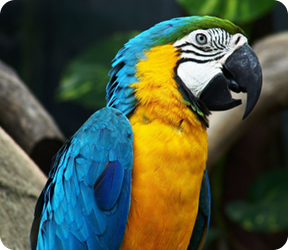
\includegraphics[width=0.9\textwidth]{figures/arara.png}\par}

\vspace{.7em}

\em Do you like araras? We do, specially our tool which shares the same name of this colorful bird.
\end{minipage}\hspace{1em}
\begin{minipage}{0.5\textwidth}
The tool name was chosen as an homage to a Brazilian bird of the same name, which is a macaw. The word \emph{arara} comes from the Tupian word \emph{a'rara}, which means \emph{big bird} (much to my chagrin, Sesame Street's iconic character Big Bird is not a macaw; according to some sources, he claims to be a golden condor). Araras are colorful, noisy, naughty and very funny. Everybody loves araras. The name seemed catchy for a tool and, in the blink of an eye, \arara\ was quickly spread to the whole \TeX\ world.
\end{minipage}
\end{messagebox}

% TODO fix reference
Now that we informally introduced rules and directives, let us take a look on how \arara\ actually works given those two elements. The whole idea is pretty straightforward, and I promise to revisit these concepts later on in this manual for an comprehensive explanation (more precisely, on Chapter~\ref{foo}).

First and foremost, we need to add at least one instruction in the source code to tell \arara\ what to do. This instruction is named \emph{directive} and it will be parsed during the preparation phase. Observe that \arara\ will tell you if no directive was found in a file, as seen in our first interaction with the tool.

An \arara\ directive is usually defined in a line of its own, started with a comment (denoted by a percent sign in \TeX\ and friends), followed by the word \abox{arara:} and task name:

\begin{codebox}{A typical directive}{teal}{\icnote}{white}
% arara: pdflatex
\documentclass{article}
...
\end{codebox}

Our example has one directive, referencing \abox{pdflatex}. It is important to observe that the \abox{pdflatex} identifier \emph{does not represent the command to be executed}, but \emph{the name of the rule associated with that directive}.

\begin{messagebox}{New feature in version 4.0}{araracolour}{\icinfo}{white}
% TODO fix reference
\textbf{Multiline directives} -- Later on in Section~\ref{foo} (page~\pageref{foo}), we will discover that a directive can also span several lines in order to provide a better code organization. For now, let us assume a typical directive occupies only one line.
\end{messagebox}

% TODO fix reference
Once \arara\ finds a directive, it will look for the associated \emph{rule}. In our example, it will look for a rule named \abox{pdflatex} which will evidently run the \abox{pdflatex} command line application. Rules are YAML files named according to their identifiers followed by the \abox{.yaml} extension and follow a strict structure. This concept is covered in Section~\ref{foo} (page~\pageref{foo}).

\begin{messagebox}{New feature in version 4.0}{araracolour}{\icattention}{white}
\textbf{REPL workflow} -- \arara\ now employs a REPL workflow for rules and directives. In previous versions, directives were extracted, their corresponding rules were analized, commands were built and added to a queue before any proper execution or evaluation. I decided to change this workflow, so now \arara\ evaluates each rule on demand, that is, there is no \emph{a priori} checking. A rule will \emph{always} reflect the current state, including potential side effects from previous executed rules. 
\end{messagebox}

Now, we have a queue of pairs $(\textit{directive}, \textit{rule})$ to process. For each pair, \arara\ will map the directive to its corresponding rule, evaluate it and run the proper command. The execution chain requires that command $i$ was successfully executed to then proceed to command $i+1$, and so forth. This is also by design: \arara\ will halt the execution if any of the commands in the queue had raised an error. How does one know if a command was successfully executed? \arara\ checks the corresponding \emph{exit status} available after a command execution. In general, a successfull execution yields 0 as its exit status.

\begin{messagebox}{New feature in version 4.0}{araracolour}{\icinfo}{white}
\textbf{Custom exit status checking} -- In previous versions, there was no way of customizing the exit status checking of a command. A command was successful if, and only if, its resulting exit status was 0 and no other value. From now on, we can define any value, or even forget about it and make it always return a valid status regardless of execution (for instance, in a rule that always is successful).
\end{messagebox}

That is pretty much how \arara\ works: directives in the source code are mapped to rules. These pairs are added to a queue. The queue is then executed and the status is reported. We will cover more details about the expansion process later on in the manual. In short, we teach \arara\ to do a task by providing a rule, and tell it to execute it through directives in the source code.

\section{Operating system remarks}
\label{sec:operatingsystemremarks}

The application was written using the Java language, so \arara\ runs on top of a Java virtual machine, available on all the major operating systems~--~in some cases, you might need to install the proper virtual machine. We tried very hard to keep both code and libraries compatible with older virtual machines or from other vendors. Currently, \arara\ is known to run on Oracle's Java 5 to 10, and OpenJDK 5 to 10. I also have reports of users sucessfully using the tool with virtual machines provided by Azul Systems, so your mileage might vary.

\begin{messagebox}{Outdated Java virtual machines}{warningcolour}{\icerror}{white}
Dear reader, beware of outdated software, mainly Java virtual machines! Although \arara\ offers support for older virtual machines, try your best to keep your software updated as frequently as possible. The legacy support exists only for historical reasons, and also due to the sheer fact that I know some people that still runs \arara\ on very old hardware. If you are not in this particular scenario, get the latest virtual machine.
\end{messagebox}

% TODO fix references
Later on in Chapter~\ref{foo} (page~\pageref{foo}), we will provide instructions on how to build \arara\ from sources using Apache Maven. Even if you use multiple operating systems, \arara\ should behave the same, including the rules. There are helper functions available in order to provide support for system-specific rule based on the underlying operating system.

\section{Support}
\label{sec:support}

If you run into any issue with \arara, please let us know. We all have very active profiles in the \href{https://tex.stackexchange.com/}{\TeX\ community at StackExchange}, so just use the \verb|arara| tag in your question and we will help you the best we can (also, take a look at their \href{https://tex.meta.stackexchange.com/q/1436}{starter guide}).  We also have a \href{https://gitter.im/cereda/arara}{Gitter chat room}, in which we occasionally hang out. Also, you if you think the report is worthy of an issue, open one in our \href{https://github.com/cereda/arara/issues}{GitHub repository}. At last, but not least, feel free to poke us by good old electronic mail (please try the other approaches first).

I really hope you like our humble contribution to the \TeX\ community. Let \arara\ enhance your \TeX\ experience, it will help you when you will need it the most. Enjoy the manual.
